\documentclass[11pt,fleqn]{article}

%% This first part is the document header, which you don't need to edit.
%% Scroll down to \begin{document}

\usepackage[latin1]{inputenc}
\usepackage{enumerate}
\usepackage[hang,flushmargin]{footmisc}
\usepackage{mdframed}
\usepackage{minted}
\usepackage{color}
\usepackage{datetime}
\usepackage{graphicx}
%%Please place all images used in documents in the images folder
\graphicspath{ {../images/} }
%% USAGE: \includegraphics[args1 = val1, args2 = val2]{filename}
\setlength{\oddsidemargin}{0px}
\setlength{\textwidth}{460px}
\setlength{\voffset}{-1.5cm}
\setlength{\textheight}{20cm}
\setlength{\parindent}{0px}
\setlength{\parskip}{10pt}

\newcommand{\mil}[2][java]{\mintinline{#1}|#2|}
%% This command allows quick use of \mintinline feature, default language is java.

%% USAGE: \mil (optional)[<language>] {content}

%% EXAMPLE: \mil[python]{if not x == 3}
%% 			\mil{if (x.equals(y)}

\begin{document}
\title{Primitive Types and Math}%Insert Title here
\author{Tim Magoun and Aravind Koneru}
\date{\textit{Compiled on} \today \hspace{1mm} at \currenttime}
\maketitle

\begin{abstract}
In this lesson we will set up your computer for Java programming, and learn about some of the primitive
types in Java. In the second half of this lesson, we will learn about the simple arithmetic operations that we'll use in the future.
\end{abstract}

\section*{Foreword}
Programming is an ever-increasingly useful skill to have in the digital world. Before learning about the
basics of Java, one must realize the following:
\begin{itemize}
\item Programming is the act of writing instructions for a computer
\item The computer could only do one thing at a time
\item Programming is supposed to make repetitive tasks easier
\item It is more important to understand the concept rather than memorizing syntax
\end{itemize}
Feel free to ask questions, they don't have to be about the current exercise.

\newpage
\section{Installing Eclipse}
Just follow the instructions on the course syllabus, which is also included below:
\begin{enumerate}
\item Go to \texttt{https://eclipse.org/downloads/eclipse-packages/}
\item Click on the corresponding installer, 32 bit or 64 bit (if you don't know the version of OS present, choose the 32 bit installer)
\item Download the installer to a known location (ex. Downloads or Desktop)
\item Execute the installer file
\item Select Eclipse IDE for Java Developers
\item Confirm install location and select preferred shortcut locations
\item Accept EULA
\item Bogosort the digits of $\pi$
\item Launch Eclipse Neon and set up preferences, line numbers are highly recommended
\end{enumerate}

\section{Creating a Java Project}
\begin{enumerate}
\item Start up Eclipse and make the workspace in a known location (ex. Documents)
\item Enter into the Java Perspective
\item Right click on \textbf{Package Explorer}, which is on the left part of the screen, and select \textbf
{New} $\rightarrow$ \textbf{Java Project}
\item Name the project \textbf{Lesson 1} and click \textbf{Finish}
\end{enumerate}

\section{The Primitive Types}
Create a new class in your \textbf{Lesson 1} project by expanding the project, right click on \textbf
{src}, and select \textbf{New} $\rightarrow$ \textbf{Class}. Name your class \textbf{PrimativeTypeExplorer} and select the check-box 
\textbf{public static void main String[] args)} under the last large text field, and `Which method stubs
would you like to create?'

Your screen should look somewhat like this:

% 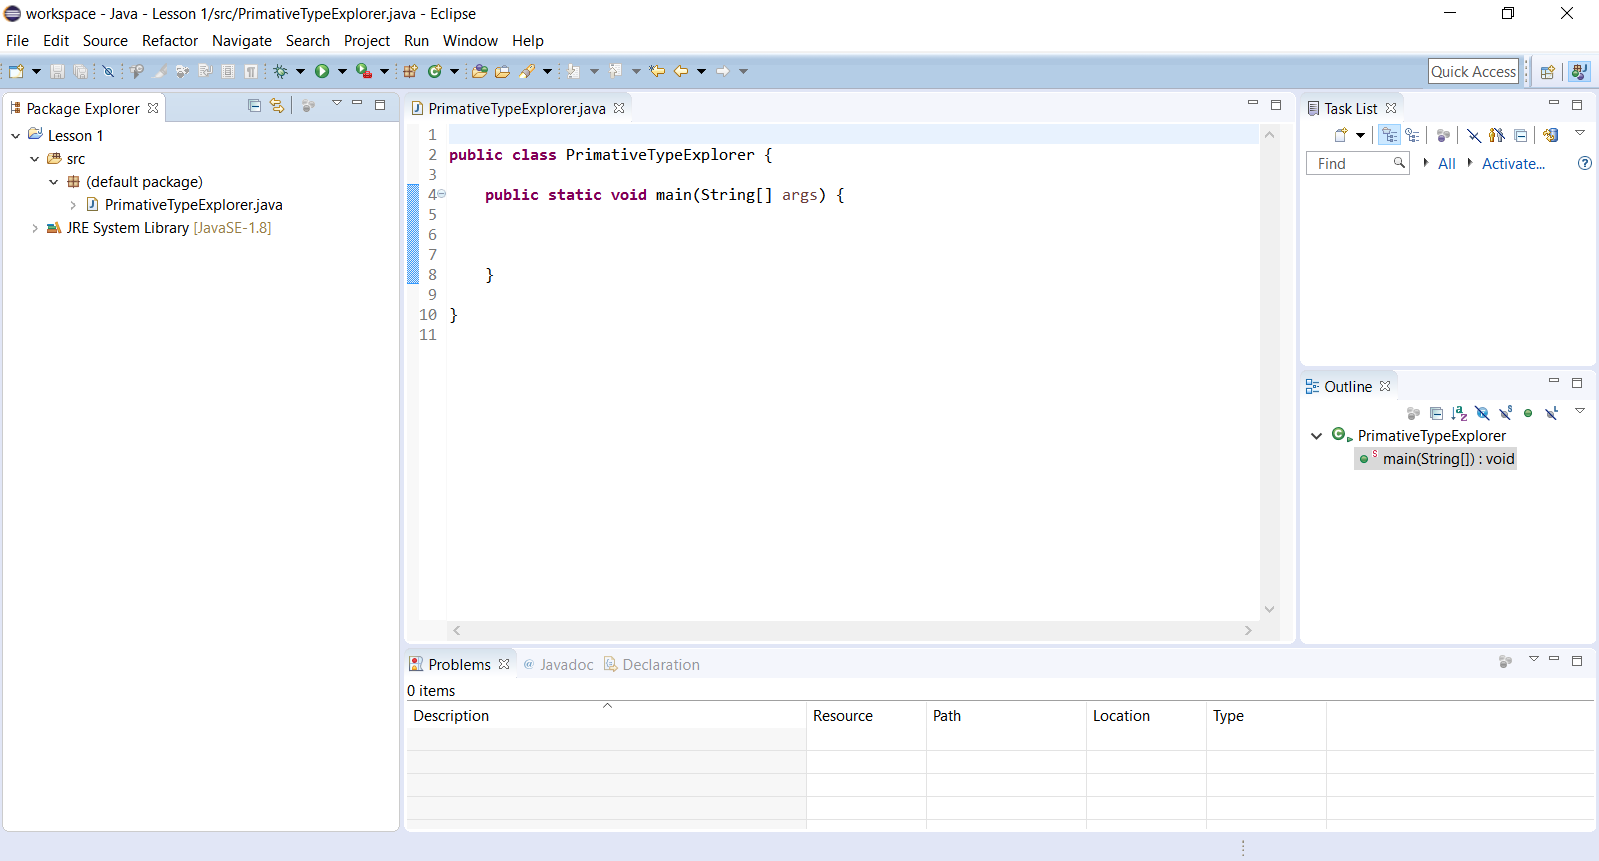
\includegraphics[scale=0.5]{Lesson_1_1.png}

\begin{center}
\section*{Variables}
\end{center}

What are variables? If you know some Algebra or Pre-Algebra, you know that
we use variables in math to represent numbers in our equations. Essentially, a
variable is an unknown value that we are trying to solve for. In programming,
variables are also used to represent values. 

In programming, we use variables all the time to store information that we would
want to access later. There are various forms of information we could store. For
example, we may want to store numbers, words, or even a variety of these things.
The type of information we want to store is usually called the
\textbf{\texttt{type}} of the variable. For example, the variable storing the
phrase ``sit vis vobiscum", would be of \texttt{type} string (in java, words are
referenced as strings). 

Some key words that you need to be aware of when discussing variables:
\begin{enumerate}
\item
\textbf{Declaration}

\item
\textbf{Initalization}

\item
\textbf{type}
\end{enumerate}

We have previous defined type, but we still need to define declaration and
initialization. 

A \textbf{declaration} is defined as the act of creating a new variable, but not
assigning it a value. In Java, we declare variables as follows:

\textit{type} name

Say that we wanted to make a variable to store an integer. We would do that by
doing:

\begin{minted}{java}
int anIntegerVariable;
\end{minted}

In this case, we have \textbf{declared} a new variable named
\texttt{anIntegerVariable} of \textbf{type} \texttt{int}. 

\textbf{Exercise}: Look at the following variables and then break down them down
like we did for \texttt{anIntegerVariable}. 

\begin{minted}{java}
    String myName;
    double pi;
    int aName;
    float someNum;
\end{minted}

So far, we have only covered how to declare a variable. This means that all of
our variables are set to \texttt{null} and we can't use them in our code. In
order to assign values to our variables we must \textbf{intialize} them. We can
initialize variables by setting them equal to some value. For example:

\begin{minted}{java}
    String myName;//declaring the variable
    myName = "Aravind";//initializing the variable
\end{minted}

We first declared the variable (\texttt{myName}) and then we assigned it the
value ``Aravind". This is an example of initalizing a variable. It is important
to note that in java, variables accept their assignments from the right. This
means that 

\begin{minted}{java}
    String myName;
    "Aravind" = myName;
\end{minted}

will throw an error. This is the case for most programming languages you will
encounter.

\textbf{Exercise}: Declare and initialize a variable for each of the following
types: 

\begin{minted}{java}
int
float
double
String
\end{minted}

It gets annoying to declare and initialize a variable on different lines. It's
much easier to do both at the same time. We can easily do this by:

\begin{minted}{java}
    int myAge = 17 //declaring and initializing a variable at the same time
\end{minted}

Note that it is common practice to declare and initialize variables on the same
line. There are situations where it may not be possible to do both, but when you
can, you should.

Now that we know about variables and how to use them, we can start doing some
basic tasks in java. I'm a strong believer in application, so many of my example
will come in the form of code. Here is the first example:

\begin{minted}{java}
int num1 = 10;
int num2 = 20;
int num3 = num1 * num2;//What are we doing here?
int num4 = num3 / num1;//Is num4 always equal to num2?
\end{minted}

In this example, we are introduced to something we haven't seen before: defining
a variable in terms of other variables. In our example, \texttt{num3} is defined
to be the product of \texttt{num1} and \texttt{num2}.Although we will always
know the numerical values of \texttt{num1} and \texttt{num2}, we won't always
know the numerical value of \texttt{num3}. Sure when \texttt{num1} and
\texttt{num2} are small, we can calculate the value of \texttt{num3}, we won't
be able to do so when \texttt{num1} and \texttt{num2} are large. The beauty of
this situation is that we always know what the value of \texttt{num3} is in
relation to that of \texttt{num1} and \texttt{num2}, but we may not always know
the numerical value. 

\textbf{Exercise}: Initialize two \texttt{String} variables with your first and
last name. Make a third variable that will store your entire name, but you must
define the third variable in terms of the first two. 





\end{document}
